\chapter{Graph Summary Precision}
\label{chap03:sec:quality}

The summary of a graph reflects the structure of that graph. Concretely, this means that all possible paths in the graph are also possible in its summary. However, this does not imply the converse, i.e., that all possible paths in a summary do exist in the graph it represents. The structure of the summary stems from the grouping of the nodes in the graph by the \gls{summarisation-relation}. Therefore, the question of the \emph{precision} of the summary with regards to the graph it represents is raised.

We judge the precision of a summary by the difference of traversing a summary or the graph it represents. Our rationale is the larger the difference, the less precise the summary is. We consider the precision of a summary with regards to the graph it represents from two directions. Firstly, we are concerned with the existence of paths in the graph. Secondly, we consider whether combinations of \gls{attributes} and/or \gls{types} in the summary do exist in the graph.

In this chapter, we present a model for measuring the precision of a summary with regards to the graph it was created from. The model rely on a summary that is set as the \emph{gold} standard, to which we compare both directions, i.e., the existence of paths and of \gls{attributes}/\gls{types} combinations.
%The quality of a summary depends on the summarisation relation used, which we discuss in terms of volume of the graph and of precision of the summarized data.

\section{Graph Summarisation Lattice}

We have introduced in Chapter~\ref{chap:summary} a framework for defining graph summaries. Each summary presented consider different properties of the graph for the \gls{summarisation-relation}, e.g., the \gls{typessummary} $R_t$ considers the type information, while the \gls{attributes-summary} $R_a$ the label of edges. Since the \glspl{summarisation-relation} consider different aspect of the graph, the nodes are grouped differently. This produces summaries of varying structure. In this chapter, we investigate how the summaries differ, whether a summary is better suited to a certain type of application that another.

In order to answer these questions, we propose a \gls{precision} which measures the amount of \emph{errors} in a summary. This model relies on the ordering of the summaries. We present in this section a partial order relation on the summaries.\\

%There exists several possible summarisation relations, each resulting in a graph summary that exhibits different properties. In the Section~\ref{chap03:sec:quality}, we discuss the impact of the relation on the \emph{precision} of a graph summary with regards to the entity graph. There is no graph summary that fits all use cases, a summary suitable for one might not be for another. In this section, we describe how various summarisation relations can be ordered into a \emph{lattice}. Thus, we can reuse previous computations where a graph summary can result from another one, instead from the entity graph.

We denote with $\sqsubseteq$ a binary relation on the set of \glspl{summarisation-relation}. It relates two summarisation relations if one can be expressed as a composition of the other.

\begin{definition}[Relation $\sqsubseteq$]
	Let $G=\left\langle V, A, l_V \right\rangle$ be a graph, $\mathcal{S}_1 = \left\langle \mathcal{W}_1, \mathcal{B}_1, l_{\mathcal{W}_1} \right\rangle$ be the summary of $G$ according to $R_1 \subseteq V \times \mathcal{W}_1$, and $\mathcal{S}_2 = \left\langle \mathcal{W}_2, \mathcal{B}_2, l_{\mathcal{W}_2} \right\rangle$ be the summary of $G$ according to $R_2 \subseteq V \times \mathcal{W}_2$.

	We say that $R_1$ precedes $R_2$, noted as $R_1 \sqsubseteq R_2$, if there exists a relation $S \subseteq \mathcal{W}_1 \times \mathcal{W}_2$ such that $R_2$ is a \emph{composition} of $R_1$ and $S$ as follows:
	$$
	R_2 = S \circ R_1 = \left\lbrace (x, z) \in V \times \mathcal{W}_2 \mid \exists y \in \mathcal{W}_1\; (x, y) \in R_1 \wedge (y, z) \in S \right\rbrace
	$$
	\label{def:partial-order}
\end{definition}

\begin{figure}
	\centering
	\resizebox{.6\textwidth}{!}{
		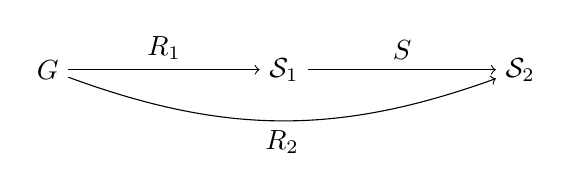
\begin{tikzpicture}[->, node distance=3cm]
\node (g) {$G$};
\node[right of = g] (g1) {$\mathcal{S}_1$};
\node[right of = g1] (g2) {$\mathcal{S}_2$};

\path
(g) edge node[above] {$R_1$} (g1)
(g1) edge node[above] {$S$} (g2)
(g) edge [bend right=20] node[below] {$R_2$} (g2)
;
\end{tikzpicture}
	}
	\caption{Summarisation relations $R_1$ and $R_2$ ordered with the binary relation $\sqsubseteq$ in Definition (\ref{def:partial-order})}
	\label{fig:partial-order}
\end{figure}

A \gls{lattice} is a \emph{partially ordered} set that contains an \emph{infimum} and a \emph{supremum}. The infimum is an element of the set that is ``smaller'', according to the partial order, than all other elements. Conversely, a supremum is an element that is ``larger'' than any other element.

We use the binary relation $\sqsubseteq$ to order the \glspl{summarisation-relation} based on their definition: two summarisation relations can be ordered if one can be expressed with the other. Figure~\ref{fig:partial-order} is a depiction of the binary relation $\sqsubseteq$ used for ordering summarisation relations. In this set, the infimum is the identity relation that maps the graph to itself, and the supremum is the relation that maps all nodes to a single sumnode.

\begin{theorem}[Graph Summarisation Lattice]
	The binary relation $\sqsubseteq$ is a \gls{partial-order}. The set of \glspl{summarisation-relation} with the partial order $\sqsubseteq$ forms a \emph{lattice} that we denote as the graph summarisation lattice.
\end{theorem}

\begin{proof}
	Let $G=\left\langle V, A, l_V \right\rangle$ be a graph, and for some set $A$, let $I_A = \left\lbrace (x, x) : x \in A \right\rbrace$ be the identity relation on $A$.
	\begin{description}
		\item[reflexivity:] Let $\mathcal{S} = \left\langle \mathcal{W}, \mathcal{B}, l_{\mathcal{W}} \right\rangle$ be the summary of $G$ according to $R \subseteq V \times \mathcal{W}$. We have $R = I_\mathcal{W} \circ R$, therefore $R \sqsubseteq R$.
		\item[antisymmetry:] For $i \in \{1, 2\}$, let $\mathcal{S}_i = \left\langle \mathcal{W}_i, \mathcal{B}_i, l_{\mathcal{W}_i} \right\rangle$ be the summary of $G$ according to $R_i \subseteq V \times \mathcal{W}_i$. If we suppose $R_1 \sqsubseteq R_2 \wedge R_2 \sqsubseteq R_1$, then $\exists S \subseteq \mathcal{W}_1 \times \mathcal{W}_2$ and $\exists T \subseteq \mathcal{W}_2 \times \mathcal{W}_1$ such that $R_2 = S \circ R_1$ and $R_1 = T \circ R_2$. By substitution, we have $R_2 = S \circ T \circ R_2$. Hence, $S \circ T = I_{\mathcal{W}_2}$. Since the identity relation is a bijection, we have a \emph{one-to-one} mapping between $\mathcal{W}_1$ and $\mathcal{W}_2$. Therefore, we have $R_1 = R_2$.
		\item[transitivity:] For $i \in \{1, 2, 3\}$, let $\mathcal{S}_i = \left\langle \mathcal{W}_i, \mathcal{B}_i, l_{\mathcal{W}_i} \right\rangle$ be the summary of $G$ according to $R_i \subseteq V \times \mathcal{W}_i$. If we suppose $R_1 \sqsubseteq R_2 \sqsubseteq R_3$, then $\exists S \subseteq \mathcal{W}_1 \times \mathcal{W}_2$ and $\exists T \subseteq \mathcal{W}_2 \times \mathcal{W}_3$ such that $R_2 = S \circ R_1$ and $R_3 = T \circ R_2$. Let $U \subseteq \mathcal{W}_1 \times \mathcal{W}_3$ be a relation defined as the composition of $S$ and $T$, i.e., $U = T \circ S$. Since the composition operation $\circ$ is associative, we have then $R_3 = U \circ R_1$. Therefore, $R_1 \sqsubseteq R_3$.
	\end{description}
	Therefore, the binary relation $\sqsubseteq$ is a partial order.
\end{proof}

The set of \glspl{summarisation-relation} can then be ordered according to $\sqsubseteq$. The Figure~\ref{fig:lattice} depicts the lattice that is formed by the partial order $\sqsubseteq$ for the \glspl{summarisation-relation} introduced in Section~\ref{sec:approximate}. For example, we remark that the \gls{typessummary} $R_t$ is smaller than the \gls{io-attributes-types-summary} $R_{ioat}$, i.e., $R_{ioat} \sqsubseteq R_t$.

\begin{remark}
The graph lattice depicts that all summaries presented in Section~\ref{sec:approximate} can be generated from the \gls{io-attributes-types-summary} $R_{ioat}$. In cases where the \gls{io-attributes-types-summary} has significantly less edges and nodes than the entity graph, this allows a more efficient computation of all summaries which summarisation relation $R$ are smaller than the latter summary, i.e., $R_{ioat} \sqsubseteq R$.
\end{remark}

\begin{figure}
	\centering
	\begin{tikzpicture}[->,>=stealth',node distance=2cm]
\node (base) {\emph{Infimum}};
\node[right of = base] (ioat) {$R_{ioat}$};
\node[right of = ioat] (ta1) {$R_{iat}$};
\node[above of = ta1] (at) {$R_{at}$};
\node[below of = ta1] (ioa) {$R_{ioa}$};
\node[right of = at] (t) {$R_t$};
\node[right of = ta1] (a) {$R_a$};
\node[right of = ioa] (a1) {$R_{ia}$};
\node[right of = t] (st) {$R_{ut}$};
\node[right of = a] (phantom) {};
\node[right of = phantom] (apex) {\emph{Supremum}};

\path
(base) edge (ioat)
(ioat) edge (ta1)
(ioat) edge (at)
(ioat) edge (ioa)
(at) edge (t)
(at) edge (a)
(ioa) edge (a)
(ioa) edge (a1)
(ta1) edge (t)
(ta1) edge (a1)
(t) edge (st)
(st) edge (apex)
(a) edge (apex)
(a1) edge (apex)
;
\end{tikzpicture}
	\caption{Lattice of the \glspl{summarisation-relation} set according to the partial order $\sqsubseteq$}
	\label{fig:lattice}
\end{figure}

\paragraph{Example.}

The Figure~\ref{fig:rel-order} depicts the sumnodes built from two summarisation relations over the graph on Figure~\ref{fig:graph}, i.e., the Types summarisation relation $R_t$ as dotted lines, and the Attributes \& Types summarisation relation $R_{at}$ as dashed lines. The solid lines represent a relation $S \subseteq \mathcal{W}_{at} \times \mathcal{W}_t$, where $\mathcal{W}_{at}$ is the set of sumnodes in the \gls{attributes-types-summary}, and $\mathcal{W}_{t}$ the sumnodes in the \gls{typessummary}.
Using the binary relation $S$, we have the order $R_{at} \sqsubseteq R_t$ between the two summarisation relations.

With the $R_{at}$ relation, the nodes $v_6$ and $v_7$ belong to different sumnodes, while they belong to the same with the $R_t$ relation. The same $R_t$ summary is built from the entity graph and from the $R_{at}$ summary. The partial order allows then to leverage pre-computed summaries in order to generate a new one.

\begin{figure}
	\centering
	\usetikzlibrary{arrows}

\begin{tikzpicture}[->,>=stealth',node distance=1.5cm,tnode/.style={node distance=2.5cm,draw,circle}]

\node[draw,circle] (0) {$v_0$};
\node[draw,circle,right of = 0] (1) {$v_1$};
\node[draw,circle,right of = 1] (2) {$v_2$};
\node[draw,circle,right of = 2] (3) {$v_3$};
\node[draw,circle,right of = 3] (4) {$v_4$};
\node[draw,circle,right of = 4] (5) {$v_5$};
\node[draw,circle,right of = 5] (6) {$v_6$};
\node[draw,circle,right of = 6] (7) {$v_7$};

\node[tnode,below left of = 0,xshift=.5cm] (ath0) {$S^{at}_0$};
\node[tnode,right of = ath0] (ath1) {$S^{at}_1$};
\node[tnode,right of = ath1] (ath2) {$S^{at}_2$};
\node[tnode,right of = ath2] (ath3) {$S^{at}_3$};
\node[tnode,right of = ath3] (ath4) {$S^{at}_4$};
\node[tnode,right of = ath4] (ath5) {$S^{at}_5$};

\node[tnode,above left of = 0,xshift=.5cm] (th0) {$\mathfrak{U}^t$};
\node[tnode,draw,circle,right of = th0] (th1) {$S^{t}_1$};
\node[tnode,draw,circle,right of = th1] (th2) {$S^{t}_2$};
\node[tnode,draw,circle,right of = th2] (th3) {$S^{t}_3$};
\node[tnode,draw,circle,right of = th3] (th4) {$S^{t}_4$};

\path
(0) edge[thick,dashed] (ath0)
(1) edge[thick,dashed] (ath1)
(2) edge[thick,dashed] (ath1)
(3) edge[thick,dashed] (ath2)
(4) edge[thick,dashed] (ath3)
(5) edge[thick,dashed] (ath3)
(6) edge[thick,dashed] (ath4)
(7) edge[thick,dashed] (ath5)

(0) edge[thick,dotted] (th0)
(1) edge[thick,dotted] (th1)
(2) edge[thick,dotted] (th1)
(3) edge[thick,dotted] (th2)
(4) edge[thick,dotted] (th3)
(5) edge[thick,dotted] (th3)
(6) edge[thick,dotted] (th4)
(7) edge[thick,dotted] (th4)

(ath0) edge[very thick] (th0)
(ath1) edge[very thick] (th1)
(ath2) edge[very thick] (th2)
(ath3) edge[very thick,bend right=5] (th3)
(ath4) edge[very thick] (th4)
(ath5) edge[very thick] (th4)
;
\end{tikzpicture}
	\caption[Ordering of graph summaries]{Sumnodes of \glspl{summarisation-relation} $R_t$ and $R_{at}$ for the graph in Figure~\ref{fig:graph}. The dashed lines represent the $R_{at}$ relation, the dotted lines the $R_t$ relation, and the solid lines the relation derived from the partial order $\sqsubseteq$, i.e., $R_{at} \sqsubseteq R_t$. The nodes with superscript $t$ belong to the summary built from $R_t$, while the nodes with superscript $at$ belong to the summary built from $R_{at}$.}
	\label{fig:rel-order}
\end{figure}

\section{Summary Error}

The confidence one may put on knowledge deduced from a summary has a more or less severe impact depending on the application. Also, the severity of an error depends on what information about the entity graph is affected by the error. In this section, we introduce a model for measuring the precision of a summary.

\subsection{Error Model}

The graph summary highlights the \emph{structure} of the entity graph. Errors in the summary boil down to the presence of invalid edges. Indeed, a path or a combination of paths may exists in the summary $\mathcal{S}$, but not in its entity graph $G$. This precision model accounts for the paths that exist in the summary but not in the entity graph.\\

%The definition of the precision model requires the introduction of an order relation on the summary. A set of summaries over a same entity graph can be ordered using the relation $\sqsubseteq$ \cite{Fernandez:1990:IEA:87626.87629}.
%For instance, if we consider the $\sim_{fbt}$ and $\sim_t$ summaries in Figures~\ref{fig:fbb-summary} and \ref{fig:classes-summary}, the nodes of $G$ in the equivalence classes $[v_1]^{\sim_{fbt}}$ and $[v_2]^{\sim_{fbt}}$ also belong to the equivalence class $[v_1]^{\sim_t}$. The equivalence classes of $\sim_{fbt}$ are then included in the equivalence classes of $\sim_t$. Therefore, the $\sim_{fbt}$-summary is inferior to the $\sim_t$-summary, noted as $\sim_{fbt} \sqsubseteq \sim_t$.
%
%\begin{definition}[$\sqsubseteq$ Ordering]
%Let $\sim_1$ and $\sim_2$ be two equivalences on an entity graph $G$. There is a partial order $\sqsubseteq$ on the $\sim_1$ and $\sim_2$ summaries, noted $\sim_1 \sqsubseteq \sim_2$, if and only if: $\forall [x]^{\sim_1} \in V^{\sim_1}, \exists [x]^{\sim_2} \in V^{\sim_2}, [x]^{\sim_1} \subseteq [x]^{\sim_2}$.
%\end{definition}

As per the recursive definition of the bisimulation summarisation relation $R_{fbt}$ presented in Section~\ref{sec:bisim-summary}, a node in the bisimulation summary \glssymbol{fbt-bisimulation-summary} refers to nodes of $G$ that share the same \emph{incoming} and \emph{outgoing} paths. Thus, the \glssymbol{fbt-bisimulation-summary} summary is the most precise summary for an entity graph with regards to the structure, i.e., all paths in the summary do exist in the original entity graph.

According to the partial order $\sqsubseteq$, the bisimulation summary \glssymbol{fbt-bisimulation-summary} of a graph $G$ is ``smaller'' than any of the other presented summaries on $G$, i.e., for any summarisation relation $R$ we have $R_{fbt} \sqsubseteq R$. Therefore, any edge on a summary can be inferred from the \glssymbol{fbt-bisimulation-summary} summary. However, the converse is not necessarily true.\\
% Relations between two $\sim$-equivalence classes can be inferred between the included $\sim_{fbt}$-equivalence classes.

We define the set $Err(R)$ as the set of inferred edges that are erroneous, i.e., the edges that do exist in a summary, but not in the entity graph. Since the summary \glssymbol{fbt-bisimulation-summary} is the most precise with regards to the structure of the entity graph, we use the summary \glssymbol{fbt-bisimulation-summary} instead of the entity graph $G$ to define the set $Err(R)$.

\begin{definition}[Summary Error $Err(R)$]
Let $G=\left\langle V, A, l_V \right\rangle$ be a graph, $\mathcal{S} = \left\langle \mathcal{W}, \mathcal{B}, l_{\mathcal{W}} \right\rangle$ be the summary of $G$ according to $R \subseteq V \times \mathcal{W}$, and $\glssymbol{fbt-bisimulation-summary} = \left\langle \mathcal{W}_{fbt}, \mathcal{B}_{fbt}, l_{\mathcal{W}_{fbt}} \right\rangle$ the bisimulation summary generated with the relation $R_{fbt}$.
The set $Err(R) \not \subset \mathcal{B}_{fbt}$ is the set of edges between nodes of \glssymbol{fbt-bisimulation-summary} that are inferred from $\mathcal{S}$ as per the $\sqsubseteq$ relation, but that do not exist in the summary \glssymbol{fbt-bisimulation-summary}.
\begin{equation*}
\begin{split}
Err(R) = \{ & (u, \alpha, v) \in \mathcal{W}_{fbt} \times \mathcal{L} \times \mathcal{W}_{fbt} \mid \\
 & \exists (x,a) \in R\; (y,b) \in R\;: (a, \alpha, b) \in \mathcal{B} \\
 & \wedge (x, u) \in R_{fbt}\; (y, v) \in R_{fbt}\; (u, \alpha, v) \not \in \mathcal{B}_{fbt} \}
\end{split}
\end{equation*}
\end{definition}

\begin{remark}
The set $Err(R)$ is equal to all possible combinations of nodes pair on $G$, keeping only the ones that exists in the summary $\mathcal{S}$ but not in the bisimulation summary \glssymbol{fbt-bisimulation-summary}.
\end{remark}

\subsubsection{Inferred Graph $\mathcal{I}(R)$}

We introduce the graph $\mathcal{I}(R)$ as the bisimulation summary \glssymbol{fbt-bisimulation-summary} that is \emph{augmented} with inferred edges from the $Err(R)$ set. This graph is used for computing the set of true and false positive edges in Section~\ref{sec:edge-precision}.

\begin{definition}[Inferred Graph]
Let $G=\left\langle V, A, l_V \right\rangle$ be a graph, $\mathcal{S} = \left\langle \mathcal{W}, \mathcal{B}, l_{\mathcal{W}} \right\rangle$ be the summary of $G$ according to $R \subseteq V \times \mathcal{W}$, and $\glssymbol{fbt-bisimulation-summary} = \left\langle \mathcal{W}_{fbt}, \mathcal{B}_{fbt}, l_{\mathcal{W}_{fbt}} \right\rangle$ be the bisimulation summary of $G$ according to $R_{fbt}$ such that $R_{fbt} \sqsubseteq R$.

We call the \emph{inferred graph} $\mathcal{I}(R) = \left\langle \mathcal{W}_{fbt}, \mathcal{C}, l_{\mathcal{W}_{fbt}} \right\rangle$ the graph which nodes and edges are those of the bisimulation summary \glssymbol{fbt-bisimulation-summary}, augmented with the edges in $Err(R)$, i.e., $\mathcal{C} = \mathcal{B}_{fbt} \cup Err(R)$.
\end{definition}

The Figure~\ref{fig:accuracy} depicts the inferred graph $\mathcal{I}(R_t)$ according to the \gls{typessummary} $\mathcal{S}_t$ in Figure~\ref{fig:classes-summary}.
Sink sumnodes are omitted for clarity. Sumnodes of the bisimulation summary \glssymbol{fbt-bisimulation-summary} are depicted with solid lines, and sumnodes of the \gls{typessummary} $\mathcal{S}_t$ with dashed lines. Edges from the $Err(R_t)$ set are represented with grey dotted arrows, while we depict sumnodes of the \gls{typessummary} with dashed arrows.\\

Given that $R_{fbt} \sqsubseteq R_t$, the nodes $S^{fbt}_1$ and $S^{fbt}_2$ are mapped to the node $S^t_1$. Similarly, the nodes $S^{fbt}_4$ and $S^{fbt}_5$ are mapped to the node $S^t_3$. Since we have that $(S^t_1, works, S^t_3) \in \mathcal{B}_t$, the edges $(S^{fbt}_1, works, S^{fbt}_5) \in Err(R_{fbt})$ and $(S^{fbt}_2, works, S^{fbt}_5) \in Err(R_{fbt})$ can be inferred, for example.

Edges from the $Err(R_t)$ set cause the nodes $S^{fbt}_1$, $S^{fbt}_5$, and $S^{fbt}_6$ to be connected. This generates the path $works.location.capital$ that exists in the \emph{Types} summary, but not in the bisimulation summary, and thus by extension, in the entity graph $G$.

\begin{figure}
	\centering
	\resizebox{\textwidth}{!}{
		\begin{tikzpicture}[->,>=stealth',node distance=4cm,every node/.style={font=\small\ttfamily}]
%Bisim
\node[draw,circle] (b0) {$S^{fbt}_0$};

\node[draw,circle,right of = b0,xshift=-.65cm] (b1) {$S^{fbt}_2$};
\node[draw,circle,right of = b0,xshift=.45cm] (b2) {$S^{fbt}_1$};

\node[draw,circle,above right of = b2,xshift=.4cm,yshift=0cm] (b3) {$S^{fbt}_3$};

\node[draw,circle,below right of = b1,xshift=1.5cm,yshift=1cm] (b4) {$S^{fbt}_4$};
\node[draw,circle,below of = b4,yshift=2.85cm] (b5) {$S^{fbt}_5$};

\node[draw,circle,below right of = b3,xshift=.5cm,yshift=0cm] (b7) {$S^{fbt}_7$};
\node[draw,circle,above right of = b4,xshift=1.6cm,yshift=-1cm] (b6) {$S^{fbt}_6$};

%Types
\node[draw,circle,dashed,ultra thick,minimum size=1.55cm,label={90:$\mathfrak{U}^t$}] (t0) {};
\node[draw,circle,dashed,ultra thick,minimum size=2.55cm,label={90:$\mathbf{S^t_1}$},right of = t0,xshift=-.15cm] (t1){};
\node[draw,circle,dashed,ultra thick,minimum size=1.55cm,label={90:$\mathbf{S^t_2}$},above right of = t1,xshift=1cm,yshift=0cm] (t2){};
\node[draw,circle,dashed,ultra thick,minimum size=2.55cm,label={90:$\mathbf{S^t_3}$},below right of = t1,yshift=.5cm,xshift=1cm] (t3){};
\node[draw,circle,dashed,ultra thick,minimum size=2.55cm,label={90:$\mathbf{S^t_4}$},right of = t1,xshift=3.65cm] (t4){};

\path[every node/.style={font=\footnotesize}]
(t0) edge[dashed,ultra thick,bend left=50] node[above] {creator} (t1)
(t0) edge[dashed,ultra thick,bend right=50] node[below] {author} (t1)
(t1) edge[dashed,ultra thick] node[fill=white] {lives} (t2)
(t1) edge[dashed,ultra thick] node[fill=white] {works} (t3)
(t2) edge[dashed,ultra thick] node[fill=white] {location} (t4)
(t3) edge[dashed,ultra thick] node[fill=white] {location} (t4)

(b0) edge[dotted,thick,gray] node[below,black,fill=white] {\emph{creator}} (b1)
(b1) edge[dotted,thick,gray,bend right=50] node[black,fill=white] {\emph{works}} (b5)
(b2) edge[dotted,thick,gray,bend right] node[black,fill=white] {\emph{works}} (b5)
(b3) edge[dotted,thick,gray,bend right] node[black,fill=white] {\emph{location}} (b7)
(b4) edge[dotted,thick,gray,bend left] node[black,fill=white] {\emph{location}} (b7)
(b5) edge[dotted,thick,gray,bend right] node[black,fill=white] {\emph{location}} (b6)
;
\end{tikzpicture}
	}
	\caption[The inferred graph $\mathcal{I}(R_t)$ created from the comparison of the Types and Bisimulation summaries]{The inferred graph $\mathcal{I}(R_t)$ based on the summaries of Figures~\ref{fig:classes-summary} and \ref{fig:fbb-summary}.
	Sink sumnodes are omitted for clarity. Sumnodes of the bisimulation summary \glssymbol{fbt-bisimulation-summary} are depicted with solid lines, and sumnodes of the \gls{typessummary} $\mathcal{S}_t$ with dashed lines. Edges from the $Err(R_t)$ set are represented with grey dotted arrows, and sumedges from the \emph{Types} summary with dashed arrows.}
	\label{fig:accuracy}
\end{figure}

\subsection{Classification of Errors}
\label{sec:error-classification}

Depending on the kind of edge in the set $Err(R)$, we identify three categories: \gls{connectivity}, \gls{attribute}, and \gls{type}. The \emph{connectivity} category reflects errors of a summary with regards to the structure of the entity graph, while the \emph{attribute} and \emph{type} categories with regards to its schema.

We illustrate the three categories in the following with regards to the \emph{Types} \glssymbol{typessummary} and \emph{Attributes} \glssymbol{attributes-summary} summaries only. Because the presented \glspl{summarisation-relation} are bigger than $R_t$ and $R_a$ as per the partial order $\sqsubseteq$, any error experienced with either $R_t$ or $R_a$ may also occur with the others.

\subsubsection{Connectivity Error $Err(R)_{con}$}

The connectivity error captures inferred paths that do not exists in the bisimulation summary \glssymbol{fbt-bisimulation-summary} but that do in the summary. For example, the Figure~\ref{fig:accuracy} depicts the inferred path $creator$ from the node $S^{fbt}_0$ to $S^{fbt}_2$.
We do not consider the sink sumnode $\varnothing$ in the connectivity error, since it doesn't provides any outgoing edge. We define $Err(R)_{con}$ as the set $Err(R)$ minus the edges leading to the sink sumnodes.

\begin{definition}[Connectivity Error]
Let $G=\left\langle V, A, l_V \right\rangle$ be a graph and $\mathcal{S} = \left\langle \mathcal{W}, \mathcal{B}, l_{\mathcal{W}} \right\rangle$ be its summary as per the summarisation relation $R \subseteq V \times \mathcal{W}$. Let $Err(R)$ be the summary error of $\mathcal{S}$. We define the connectivity error set $Err(R)_{con}$ as follows:

$$
Err(R)_{con} = \left\lbrace (x, \alpha, y) \in Err(R) \mid y \neq \varnothing \right\rbrace
$$
\end{definition}

\subsubsection{Attribute Error $Err(R)_{attr}$}

The attribute error captures edges from the summary error set $Err(R)$ that have an impact on the schema of the entity graph, due to additional \gls{attributes} inferred by the summary. For example, the node $S^t_4$ in Figure~\ref{fig:classes-summary} implies the existence of a node in $G$ with edges $capital$ and $label$, which is however not the case. We define $Err(R)_{attr}$ as the set that contains edges of $Err(R)$ in which the attribute is not in the set $\gls{attributes}(x)$ of the node $x$.

\begin{definition}[Attribute Error]
	Let $G=\left\langle V, A, l_V \right\rangle$ be a graph, $\mathcal{S} = \left\langle \mathcal{W}, \mathcal{B}, l_{\mathcal{W}} \right\rangle$ be the summary of $G$ according to $R \subseteq V \times \mathcal{W}$, and $\glssymbol{fbt-bisimulation-summary} = \left\langle \mathcal{W}_{fbt}, \mathcal{B}_{fbt}, l_{\mathcal{W}_{fbt}} \right\rangle$ be the bisimulation summary of $G$ according to $R_{fbt}$. Let $Err(R)$ be the summary error of $\mathcal{S}$. We define the attribute error set $Err(R)_{attr}$ as follows:

	$$
	Err(R)_{attr} = \left\lbrace (x, \alpha, y) \in Err(R) \mid \alpha \not \in \gls{attributes}(x) \right\rbrace
	$$
	where
	$$
	\gls{attributes}(x \in \mathcal{W}_{fbt}) = \left\lbrace \alpha \mid \exists y \in \mathcal{W}_{fbt} (x, \alpha, y) \in \mathcal{B}_{fbt} \right\rbrace
	$$
\end{definition}

\subsubsection{Type Error $Err(R)_{type}$}

The type error captures edges from the summary error set $Err(R)$ that impact on the schema of the entity graph, due to additional types inferred from the summary.
For example, in the Figure~\ref{fig:attributes-summary} the node $S^a_2$ contains the nodes $\left\lbrace v_3, v_4, v_5 \right\rbrace$, since all three have the same set of \gls{attributes}, i.e., $label$, $location$ and $a$. Then, we may infer from that node the possible existence of a node in $G$ with types $Place$ and $City$, which is however not the case. We define $Err(R)_{type}$ as the set that contains additional types inferred from $Err(R)$, i.e., a type attribute $(x, \glssymbol{atype}, y) \in Err(R)$, in which the target $y$ is not in the set $types(x)$ of the node $x$.

\begin{definition}[Type Error]
	Let $G=\left\langle V, A, l_V \right\rangle$ be a graph, $\mathcal{S} = \left\langle \mathcal{W}, \mathcal{B}, l_{\mathcal{W}} \right\rangle$ be the summary of $G$ according to $R \subseteq V \times \mathcal{W}$, and $\glssymbol{fbt-bisimulation-summary} = \left\langle \mathcal{W}_{fbt}, \mathcal{B}_{fbt}, l_{\mathcal{W}_{fbt}} \right\rangle$ be the bisimulation summary of $G$ according to $R_{fbt}$. Let $Err(R)$ be the summary error of $\mathcal{S}$. We define the type error set $Err(R)_{type}$ as follows:

	$$
	Err(R)_{type} = \left\lbrace (x, \glssymbol{atype}, y) \in Err(R) \mid y \not \in types(x) \right\rbrace
	$$
	where
	$$
	types(x \in \mathcal{W}_{fbt}) = \left\lbrace \l_{\mathcal{W}_{fbt}}(c) \mid \exists c \in \mathcal{W}_{fbt} (x, \glssymbol{atype}, c) \in \mathcal{B}_{fbt} \right\rbrace
	$$
\end{definition}

\subsection{Sumedge Precision}
\label{sec:edge-precision}

If we were to traverse the inferred graph $\mathcal{I}(R)$, we can follow sumedges of the $\mathcal{B}_{fbt}$ set from the bisimulation summary \glssymbol{fbt-bisimulation-summary}, but also from the summary error set $Err(R)$. The former sumedges are \emph{true positive} sumedges, while the latter are \emph{false positive} sumedges.

Our rationale is that following sumedges from the first set can be reflected on the entity graph by following an instance of that summary path, hence it is a true positive sumedge. On the contrary, following a sumedge from the summary error set can not be reflected on the entity graph since there are no instances of that summary path that forms an existing edge.\\

We define the true positive sumedges for a given sumnode as its outgoing sumedges that belong to the bisimulation summary.

\begin{definition}[True Positive Sumedges]
Let $G=\left\langle V, A, l_V \right\rangle$ be a graph and $\glssymbol{fbt-bisimulation-summary} = \left\langle \mathcal{W}_{fbt}, \mathcal{B}_{fbt}, l_{\mathcal{W}_{fbt}} \right\rangle$ be the bisimulation summary of $G$ according to summarisation relation $R_{fbt}$.
The set of true positive sumedges is defined as follows:
$$
TP(x \in \mathcal{W}_{fbt}) = \{ (\alpha, y) \in \mathcal{L} \times \mathcal{W}_{fbt} \mid (x, \alpha, y) \in \mathcal{B}_{fbt} \}
$$
\end{definition}

We define the false positive sumedges for a given sumnode with regards to a summarisation relation $R$ as its outgoing sumedges that belong to the summary error set $Err(R)$.

\begin{definition}[False Positive Sumedges]
Let $G=\left\langle V, A, l_V \right\rangle$ be a graph, $\mathcal{S} = \left\langle \mathcal{W}, \mathcal{B}, l_{\mathcal{W}} \right\rangle$ be the summary of $G$ according to $R \subseteq V \times \mathcal{W}$, and $\glssymbol{fbt-bisimulation-summary} = \left\langle \mathcal{W}_{fbt}, \mathcal{B}_{fbt}, l_{\mathcal{W}_{fbt}} \right\rangle$ be the bisimulation summary of $G$ according to $R_{fbt}$.
$$
FP(R, x \in \mathcal{W}_{fbt}) = \{ (\alpha, y) \in \mathcal{L} \times \mathcal{W}_{fbt} \mid (x, \alpha, y) \in Err(R) \}
$$
\end{definition}

We define $Prec(R, x)$ the \emph{edge precision} of a sumnode of the bisimulation summary $x \in \mathcal{W}_{fbt}$ with regards to a summarisation relation $R$ as the proportion of the true positives over all the positive sumedges.

\begin{definition}[Sumedge Precision]
Let $G=\left\langle V, A, l_V \right\rangle$ be a graph, $\mathcal{S} = \left\langle \mathcal{W}, \mathcal{B}, l_{\mathcal{W}} \right\rangle$ be the summary of $G$ according to $R \subseteq V \times \mathcal{W}$, and $\glssymbol{fbt-bisimulation-summary} = \left\langle \mathcal{W}_{fbt}, \mathcal{B}_{fbt}, l_{\mathcal{W}_{fbt}} \right\rangle$ be the bisimulation summary of $G$ according to $R_{fbt}$.
$$
Prec(R, x) = \frac{\vert TP(x) \vert}{\vert TP(x) \bigcup FP(R, x) \vert}
$$
\end{definition}

The sets $TP(x)$ and $FP(x)$ contain the true and false positive edges which source is $x$, respectively. For example, in Figure~\ref{fig:accuracy}, the edge $(S^{fbt}_0, creator, S^{fbt}_1)$ is in $TP(x)$, since it does exist in the bisimulation summary \glssymbol{fbt-bisimulation-summary}. The edge $(S^{fbt}_0, creator, S^{fbt}_2)$ is in $FP(x)$, since it does not exist in \glssymbol{fbt-bisimulation-summary}. In total, this results that $Prec\left(R, S^{fbt}_0\right) = \frac{3}{4}$.

The \emph{probability interpretation} of $Prec(R, x)$ is the probability that a randomly selected edge is correctly summarised. We note the recall is always equal to $1$, since there is no false negative edges in the presented \glspl{summarisation-relation}.\\

We use $Prec(R, x)$ as the precision measure for each of the classification of errors. We note that for a same node, the edge precision may vary between the three categories. As an example, consider the node $S^{fbt}_0$ in Figure~\ref{fig:accuracy}. The edge attribute precision is equal to $0$, since the \gls{attributes} in both \glssymbol{fbt-bisimulation-summary} and $\mathcal{I}(R_t)$ summaries for this node are $creator$ and $author$. However, the connectivity precision is equal to $\frac{3}{4}$.
